The CSCs in the muon endcap were designed to overlap slightly along
their edges, such that a track passing through the narrow ``overlap
regions'' would be observed by both of the neighboring chambers,
without scattering volumes in between or propagation over large
distances.  These tracks can therefore measure the relative alignment
of the pairs of chambers they connect with high precision.  All endcap
rings except for ME1/3 are connected in this way by overlaps.  In this
section, we will describe a method to align CSCs within each ring with
only a small sample of tracks and demonstrate the accuracy of the
method by comparing its results with an independent measurement.

\subsection{Overlap Method Algorithm} 

The basic strategy is to measure differences in alignment parameters
for pairs of chambers and then propagate alignment corrections azimuthally around
the ring by solving a system of equations.  Relative alignment
corrections between overlapping neighboring chambers $i$ and $i+1$ are derived
from the consistency of track segments with a single, straight line.

At each interface between two overlapping chambers, we fit hits in the 6 layers of
each chamber to straight lines $r\phi_i(z) = a_i + b_i z$ and
$r\phi_{i+1}(z) = a_{i+1} + b_{i+1} z$ in a shared coordinate system
and then propagate these segments to a plane equidistant between the
two chambers (at $z=0$).  The position-matching residual on the
plane is $\Delta a = a_i - a_{i+1}$ and the angle-matching residual
is $\Delta b = b_i - b_{i+1}$.  The overlap region is a thin strip
spanning the chamber only along the $y$ dimension, so we can consider
fitting these residuals as a function of the track's $y$ intersection
with the plane of comparison (a linear fit of linear track-fits).
We therefore have access to four types of residuals:
\begin{itemize}
\item $\Delta a(y=0)$: the relative $\delta_{r\phi}$
correction in position along a circle centered on the beamline,
\item $\Delta b(y=0)$: the relative $\delta_{\phi_y}$
angle between the two chambers,
\item $\frac{\partial}{\partial y} \Delta a(y)$: the relative $\delta_{\phi_z}$ angle,
\item $\frac{\partial}{\partial y} \Delta b(y)$: a non-rigid twist of the chambers.
\end{itemize}
We consider only the three alignment corrections ($\delta_{r\phi}$,
$\delta_{\phi_y}$, and $\delta_{\phi_z}$), presented graphically in
Figure~\ref{fig:overlaps_parameters}.

\begin{figure}
\subfigure[$\delta_{\phi_y}$ from $\Delta b(y=0)$]{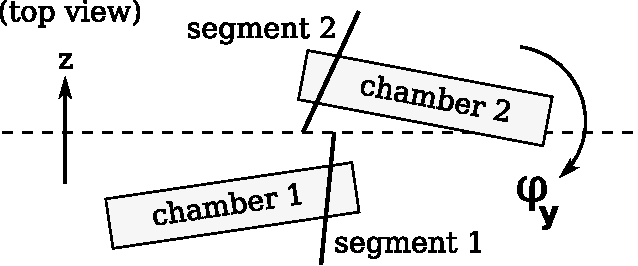
\includegraphics[width=0.33\linewidth]{plots/csc_overlaps_alignment/topview_1.pdf}} \hfill \subfigure[$\delta_{r\phi}$ from $\Delta a(y=0)$]{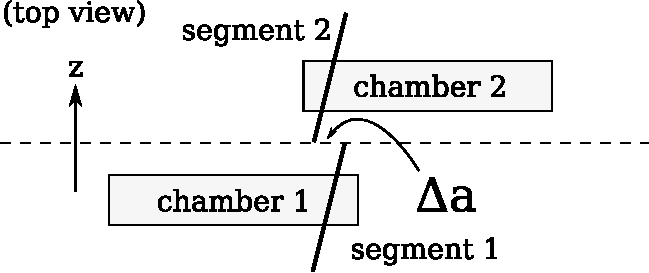
\includegraphics[width=0.33\linewidth]{plots/csc_overlaps_alignment/topview_2.pdf}} \hfill \subfigure[$\phi_z$ from $\frac{\partial}{\partial y} a(y)$]{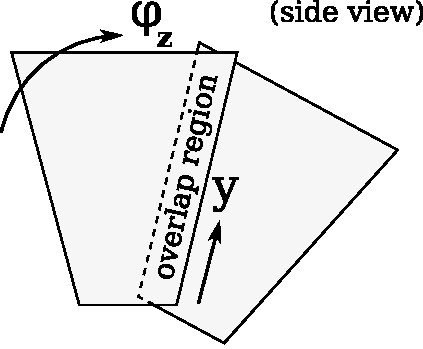
\includegraphics[width=0.18\linewidth]{plots/csc_overlaps_alignment/sideview.pdf}}
\caption{How three track parameters are determined from linear fits to $\Delta a(y)$ and $\Delta b(y)$, where $\Delta a$ and $\Delta b$ are the positions and slopes of track segments at a plane between the two CSCs.  \label{fig:overlaps_parameters}}
\end{figure}

While it is possible to resolve all three corrections at once, note
that $\delta_{\phi_y}$ is independent of the other two and
$\delta_{r\phi}$ is independent of $\delta_{\phi_z}$.  We can
therefore ignore dependencies if we align the parameters in the
following order: $\delta_{\phi_y}$, then $\delta_{r\phi}$, and then
$\delta_{\phi_z}$.

The problem of propagating alignment corrections around the ring is
identical for each of the three parameters, so we will present it only
once in an abstract way.  Label the mean of each residuals
distribution $\alpha_{i\mbox{\scriptsize, }i+1}$ (for each of the
three types of residuals under consideration) with $A_i$ and $A_{i+1}$
being the alignment corrections for the neighboring chambers
($\delta_{\phi_y}$, $\delta_{r\phi}$, or $\delta_{\phi_z}$).  Each
ring has $N$ = 18 or 36 chambers, so $i$ ranges from 1 to $N$ with the
convention that $N+1 = 1$ (to close the loop).

If we move chamber $i$ and $i+1$ by $A_i$ and $A_{i+1}$, the mean of
the residuals between them can be expected to change by $(A_i -
A_{i+1})$.  To optimize all of the residuals at once, we define a
$\chi^2$ as
\begin{equation}
\chi^2 = (\alpha_{12} - A_1 + A_2)^2 + (\alpha_{23} - A_2 + A_3)^2 + \ldots + (\alpha_{N1} - A_N + A_1)^2
\end{equation}
and minimize it by setting its derivatives to zero.  For example,
\begin{equation}
\frac{1}{2} \frac{\partial \chi^2}{\partial A_2} = (\alpha_{12} - A_1 + A_2) - (\alpha_{23} - A_2 + A_3) = 0 \mbox{.}
\end{equation}
A complete set of such equations, written in matrix form, looks like
the following:
\begin{equation}
\left(\begin{array}{c}
\alpha_{1,2} - \alpha_{N,1} \\
\alpha_{2,3} - \alpha_{1,2} \\
\vdots \\
\alpha_{(N-1),N} - \alpha_{(N-2),(N-1)} \\
\alpha_{N,1} - \alpha_{(N-1),N}
\end{array} \right)
=
\left(\begin{array}{r r r r r}
2 & -1 &  &  & -1 \\
-1 & 2 & -1 &  &  \\
 &  & \ddots & &  \\
 &  & -1 & 2 & -1 \\
-1 &  &  & -1 & 2
\end{array}\right)
\left(\begin{array}{c}
A_1 \\
A_2 \\
\vdots \\
A_{N-1} \\
A_N \\
\end{array} \right)\mbox{.}
\label{eqn:NbyNmatrix}
\end{equation}
To align all $N$ chambers, we need only invert this $N\times N$
matrix, and $N$ is small enough to be manageable.

Unfortunately, the matrix in Equation~\ref{eqn:NbyNmatrix} is singular
because a relative alignment procedure cannot determine the global
position of the whole system.  Rotating the whole ring rigidly by
adding the same constant to every $A_i$ would leave the $\chi^2$
invariant.  This is a flat direction in ($A_1$, $A_2$, \ldots\ $A_N$)
space, and it can be unflattened by preferring the corrections $A_i$
to be as small as possible.  We add the average of $A_i$
\begin{equation}
\left[ \frac{1}{N} \left(A_1 + A_2 + \ldots + A_N\right) \right]^2
\label{eqn:average}
\end{equation}
to the $\chi^2$ so that it will be minimized, and each derivative
equation becomes
\begin{equation}
\frac{1}{2} \frac{\partial \chi^2}{\partial A_i} = (\alpha_{i-1\mbox{\scriptsize, }i} - A_{i-1} + A_i) - (\alpha_{i\mbox{\scriptsize, }i+1} - A_i + A_{i+1}) + \frac{1}{N^2} \sum_{i=1}^N A_i = 0 \mbox{.}
\end{equation}
The right-hand-side of Equation~\ref{eqn:NbyNmatrix} becomes
\begin{equation}
\left[\left(\begin{array}{r r r r r}
2 & -1 &  &  & -1 \\
-1 & 2 & -1 &  &  \\
 & & \ddots & &  \\
 &  & -1 & 2 & -1 \\
-1 &  &  & -1 & 2
\end{array}\right)
+
\frac{1}{N^2}
\left(\begin{array}{r r r r r}
1 & 1 & \cdots &   & 1 \\
1 & 1 &   &   &   \\
\vdots &   & \ddots &   &   \\
  &   &   &   &   \\
1 &   &   &   & 1
\end{array}\right)
\right]
\left(\begin{array}{c}
A_1 \\
A_2 \\
\vdots \\
A_4 \\
A_5 \\
\end{array} \right)\mbox{.}
\label{eqn:solution}
\end{equation}
It has a unique solution in which the average of $A_i$ is exactly
zero.

The circular ring of chambers also provides an internal cross-check:
the closure
\begin{equation}
\sum_{i=1}^N \alpha_{i\mbox{\scriptsize, }i+1} - (A_i - A_{i+1}) = \sum_{i=1}^N \alpha_{i\mbox{\scriptsize, }i+1}
\end{equation}
must be zero.  The closure is independent of alignment, because all
$A_i$ terms cancel in the sum.  A non-zero closure would indicate an
incorrect circumference for the ring, either from our description of
the chamber widths or their radial distance from the beamline.  All
measured values of closure were consistent with zero.

This algorithm can be extended to align layers within the CSC
chambers, taking advantage of the two-chamber overlap to resolve
ambiguities between track-fitting and layer alignment in an isolated
chamber.  In the 2008 LHC beam-halo run, many layer measurements were
not statistically significant, with a precision of 50--100~$\mu$m, so
we do not present the results here.

\subsection{Monte Carlo Study}

The procedure was first applied to simulated beam-halo with
approximately the same number of events as the 2008 LHC run.  The
azimuthal and radial distributions are not exactly the same as in
data, as they are notoriously difficult to predict for a new
accelerator.  Starting from a misaligned detector, the procedure
re-aligned $\delta_{\phi_y}$ with about 1~mrad precision,
$\delta_{r\phi}$ with about 230~$\mu$m, and $\delta_{\phi_z}$ with
about 0.25~mrad, by comparison with the true positions of the
chambers, known in simulation.  Figure~\ref{fig:overlaps_mc}
shows histograms of the differences between aligned values of the
parameters and their true values.

\begin{figure}
\subfigure[$\delta_{\phi_y}$ precision is $\sim$1~mrad]{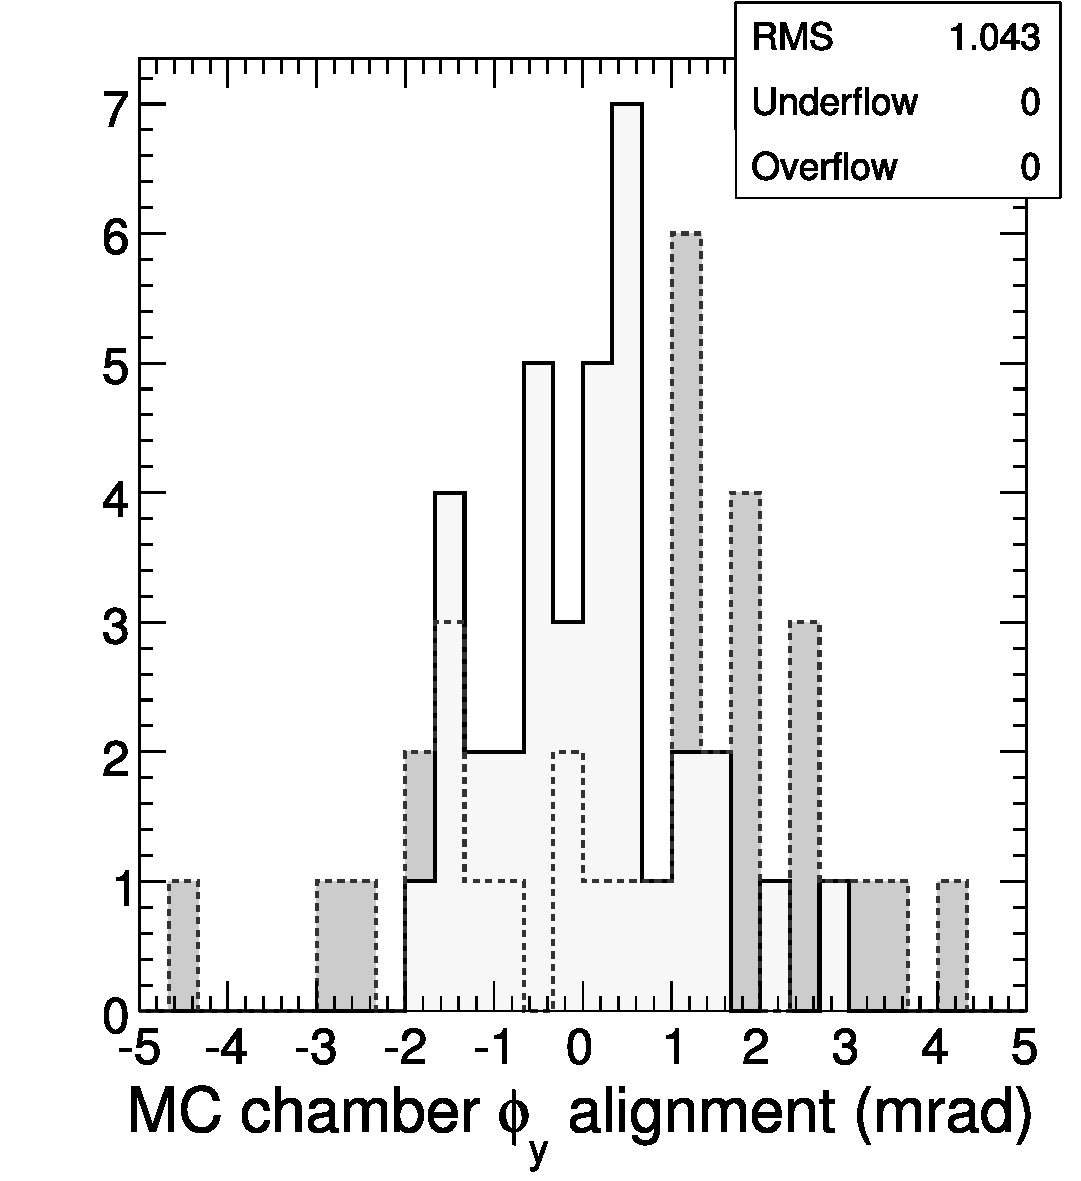
\includegraphics[width=0.3\linewidth]{plots/csc_overlaps_alignment/mcchamber_phiy.pdf}} \hfill \subfigure[$\delta_{r\phi}$ precision is $\sim$230~$\mu$m]{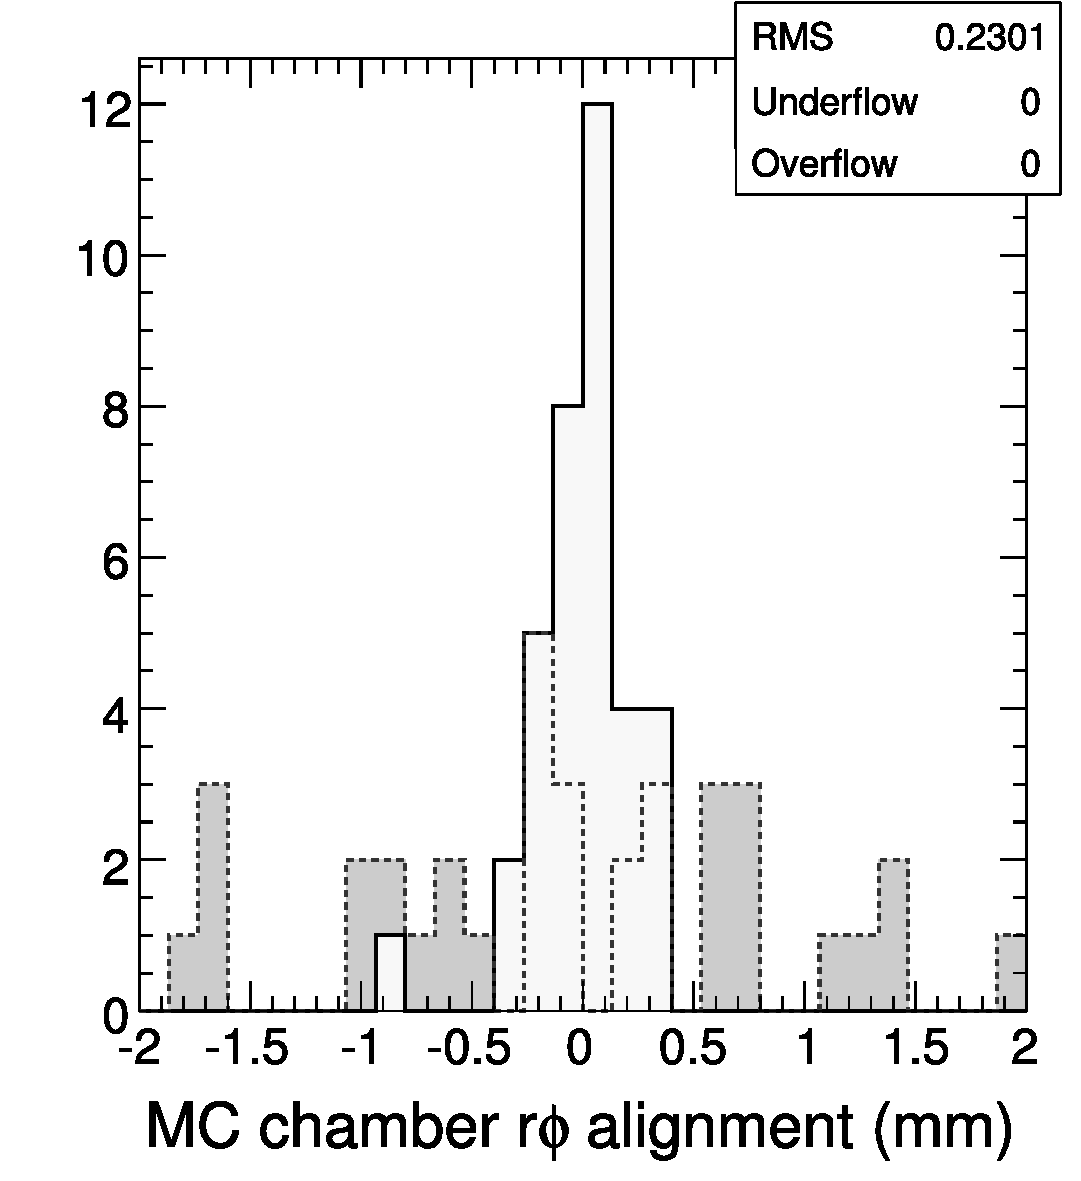
\includegraphics[width=0.3\linewidth]{plots/csc_overlaps_alignment/mcchamber_rphi.pdf}} \hfill \subfigure[$\delta_{\phi_z}$ precision is $\sim$0.25~mrad]{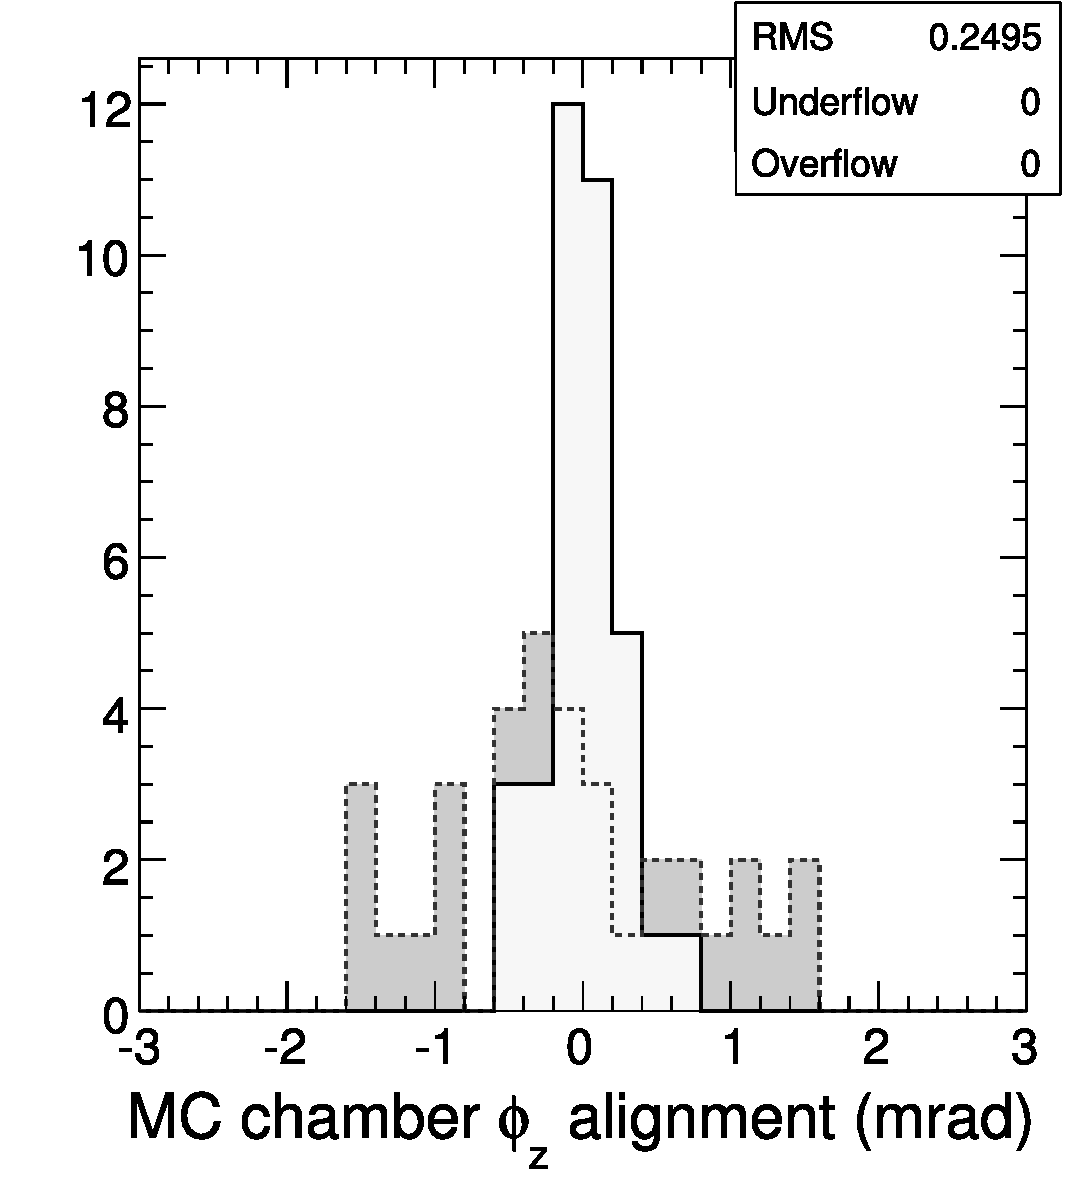
\includegraphics[width=0.3\linewidth]{plots/csc_overlaps_alignment/mcchamber_phiz.pdf}} \hfill
\caption{Comparison of CSC alignment parameters with their true values before (dark) and after (light) a simulated beam-halo alignment with similar statistics to the 2008 LHC run. \label{fig:overlaps_mc}}
\end{figure}

\subsection{Alignment Results}

In September of 2008, protons circulated in beam-2 of the LHC tunnel
for 9~minutes, and enough data were collected to test the CSC Overlaps
procedure.  More beam-halo muons illuminated the inner rings (ring~1)
of the minus side of the endcap because beam-halo muons tend to be close to
the beamline and beam-2 passed through CMS in the direction from $-z$ toward $+z$.  At
that time, all chambers in ME$-$2/1 and ME$-$3/1 were operational, so
we aligned them with the CSC Overlaps algorithm.

To verify the aligned positions, we compare them with photogrammetry
measurements.  Each chamber has two reflective alignment targets whose
positions can be measured with 300~$\mu$m precision by photographing
them in a strong light.  From these, $\delta_{r\phi}$ and
$\delta_{\phi_z}$ corrections (relative to the design geometry) can be
computed with $\mbox{(300~$\mu$m)}/\sqrt{2} = 210$~$\mu$m and
$\mbox{(300~$\mu$m)} \cdot \sqrt{2} / \ell = 0.23$~mrad precision,
respectively (where $\ell$ is half the distance between photogrammetry
targets, about 1.9~m in this case).  Errors from $\phi_y$
misalignments are negligible in these transformations.  The
photogrammetry and track-based measurements were both taken with the
CMS solenoid turned off.  (The solenoid's field is strong enough to
move the chambers, invalidating the measurement.)  Unlike
photogrammetry, the track-based measurement can also be performed with
the solenoid on, though no such data were taken while LHC beam-halo muons
could be collected.

In Figure~\ref{fig:overlaps_data1}, the track-based and photogrammetry
corrections to ideal geometry are presented.  Both yield significant
deviations from zero, yet agree rather well.  We plot the same
data as histograms of differences between track-based and
photogrammetry measurements in Figure~\ref{fig:overlaps_data2}, and
observe that the widths of these distributions are 340~$\mu$m and
0.42~mrad.  Subtracting the
photogrammetry uncertainties in quadrature from standard deviations
observed in the plots,
\begin{eqnarray}
\mbox{track-based $\delta_{r\phi}$ accuracy} &=& \sqrt{(\mbox{340~$\mu$m})^2 - (\mbox{210~$\mu$m})^2} = \mbox{270~$\mu$m} \\
\mbox{track-based $\phi_z$ accuracy} &=& \sqrt{(\mbox{0.42~mrad})^2 - (\mbox{0.23~mrad})^2} = \mbox{0.35~mrad,}
\end{eqnarray}
in rough agreement with the simulation's prediction and close to the
scale of the intrinsic hit resolution of the detectors (116~$\mu$m).  Assuming that
the errors are statistical, an hour or more of similar tracks would
yield an alignment that is more precise than the intrinsic hit resolution.

\begin{figure}
\begin{center}
\begin{minipage}{\linewidth}
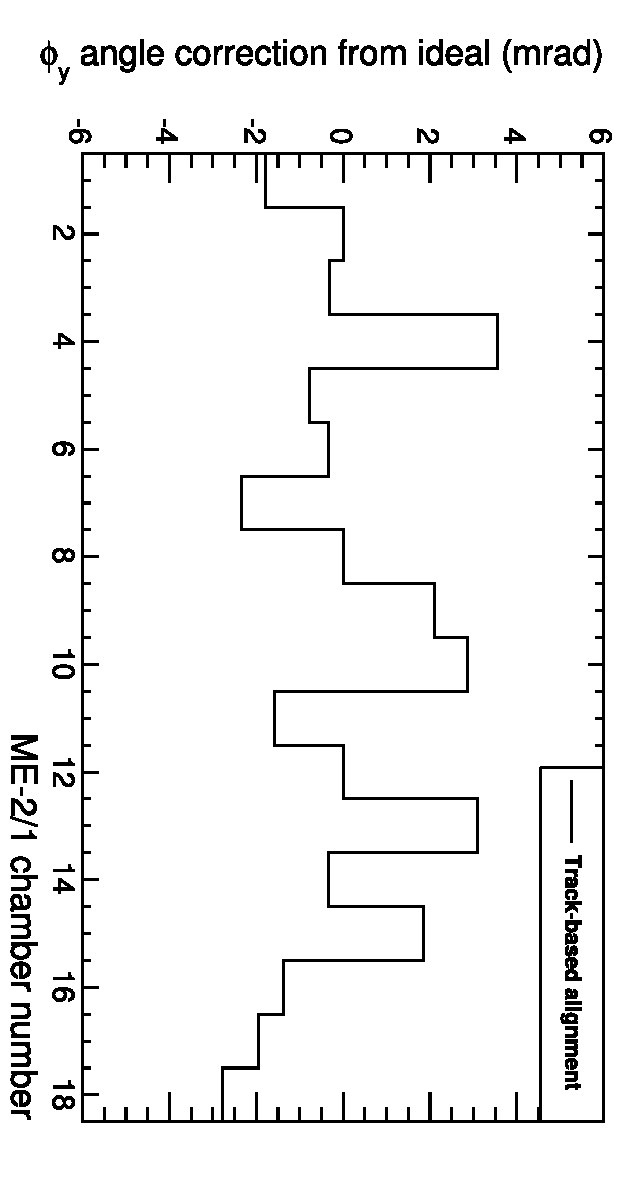
\includegraphics[height=0.48\linewidth, angle=90]{plots/csc_overlaps_alignment/compare_m21_phiy.pdf} 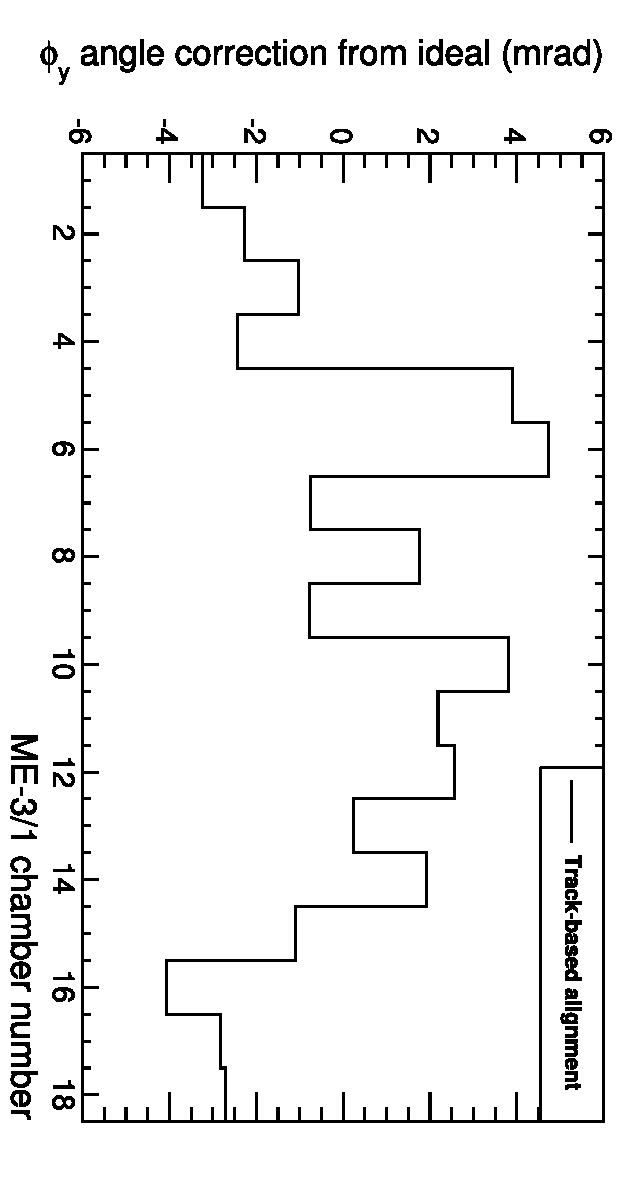
\includegraphics[height=0.48\linewidth, angle=90]{plots/csc_overlaps_alignment/compare_m31_phiy.pdf}

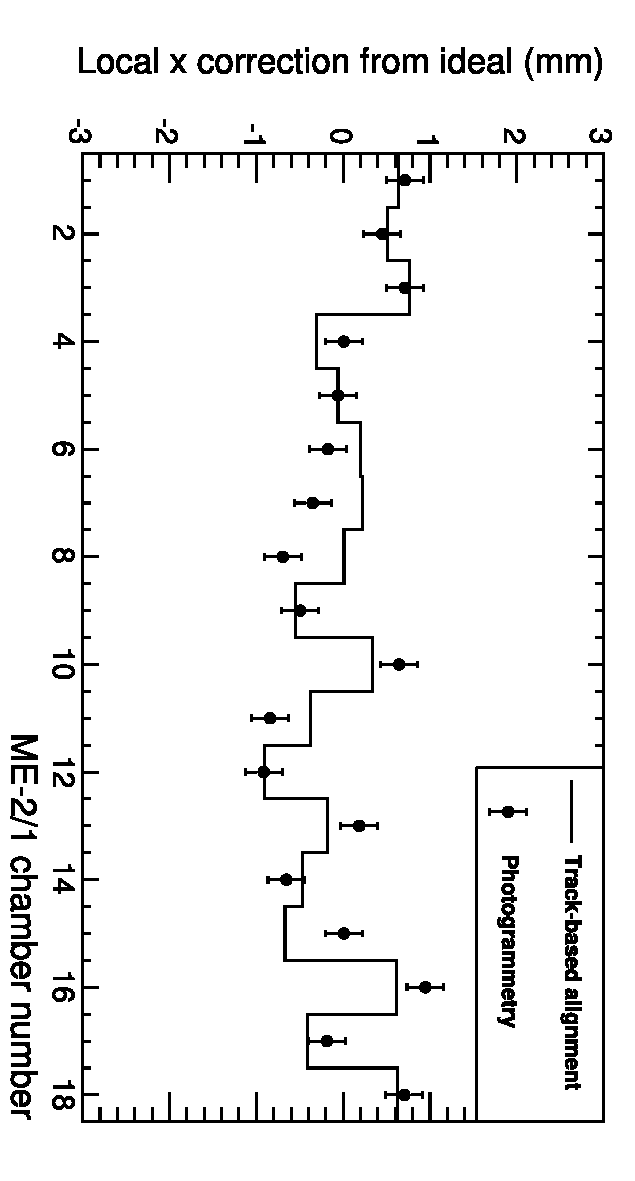
\includegraphics[height=0.48\linewidth, angle=90]{plots/csc_overlaps_alignment/compare_m21_x.pdf} 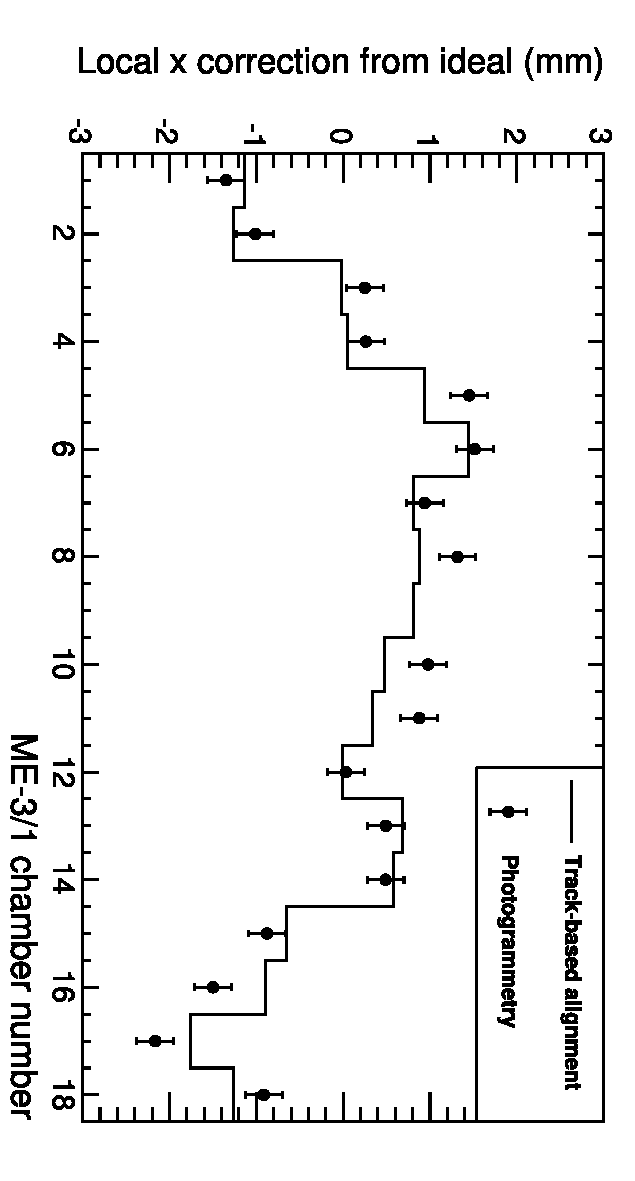
\includegraphics[height=0.48\linewidth, angle=90]{plots/csc_overlaps_alignment/compare_m31_x.pdf}

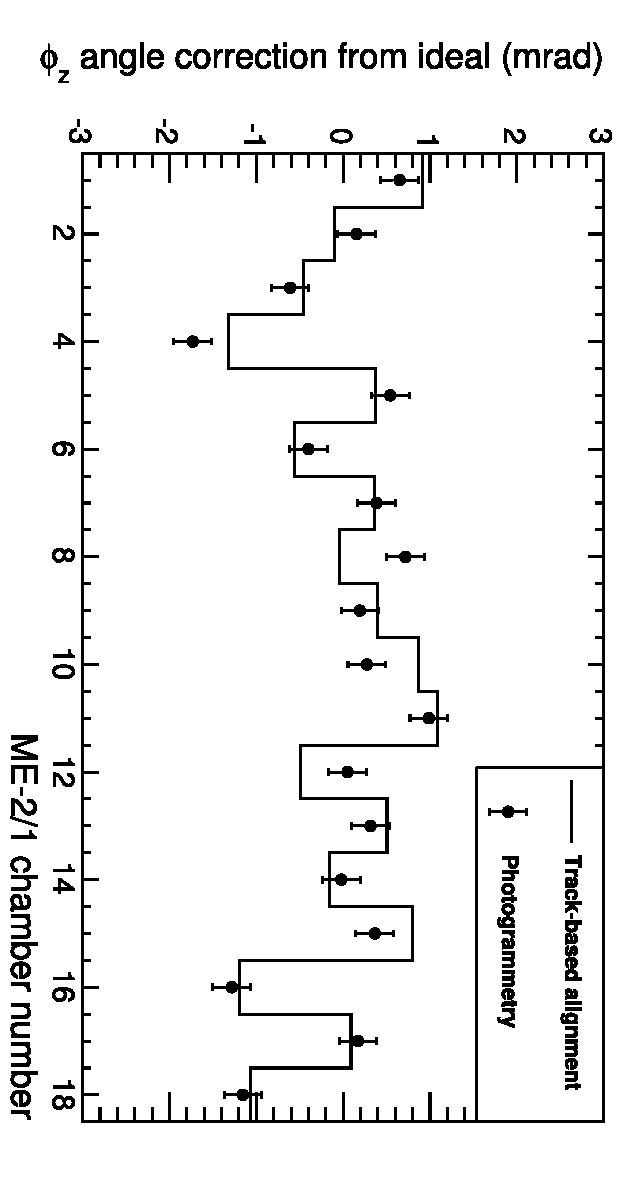
\includegraphics[height=0.48\linewidth, angle=90]{plots/csc_overlaps_alignment/compare_m21_phiz.pdf} 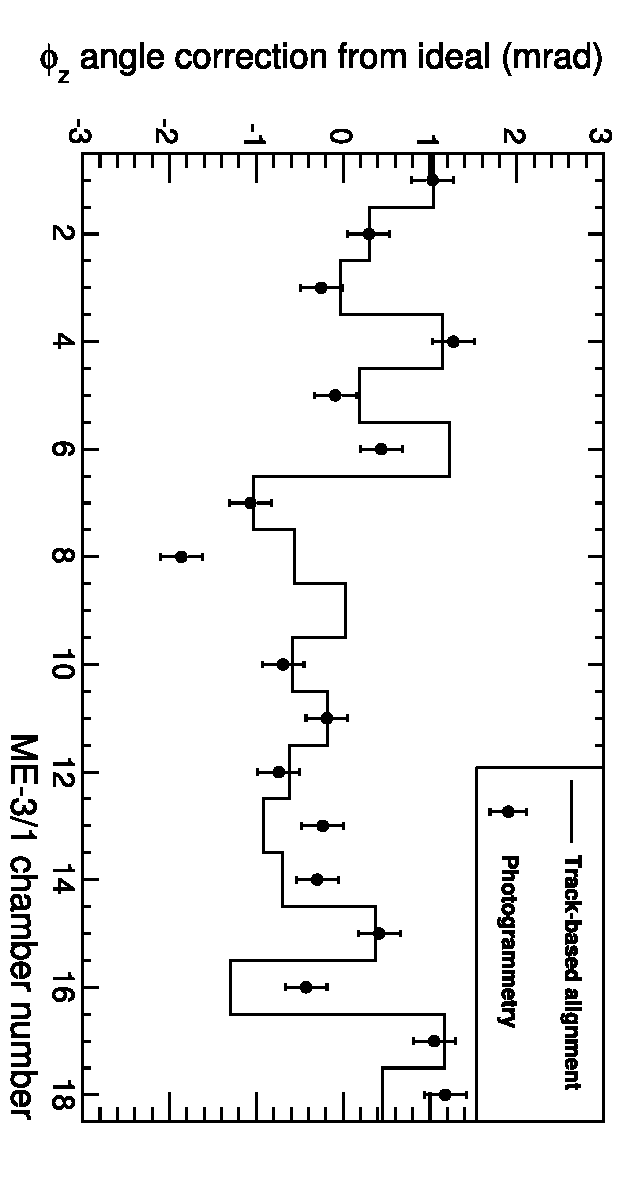
\includegraphics[height=0.48\linewidth, angle=90]{plots/csc_overlaps_alignment/compare_m31_phiz.pdf}
\end{minipage}
\end{center}
\caption{CSC alignment results from the Overlaps procedure and the 2008 LHC run, presented as a difference from ideal and compared with photogrammetry where possible. \label{fig:overlaps_data1}}
\end{figure}

\begin{figure}
\begin{center}
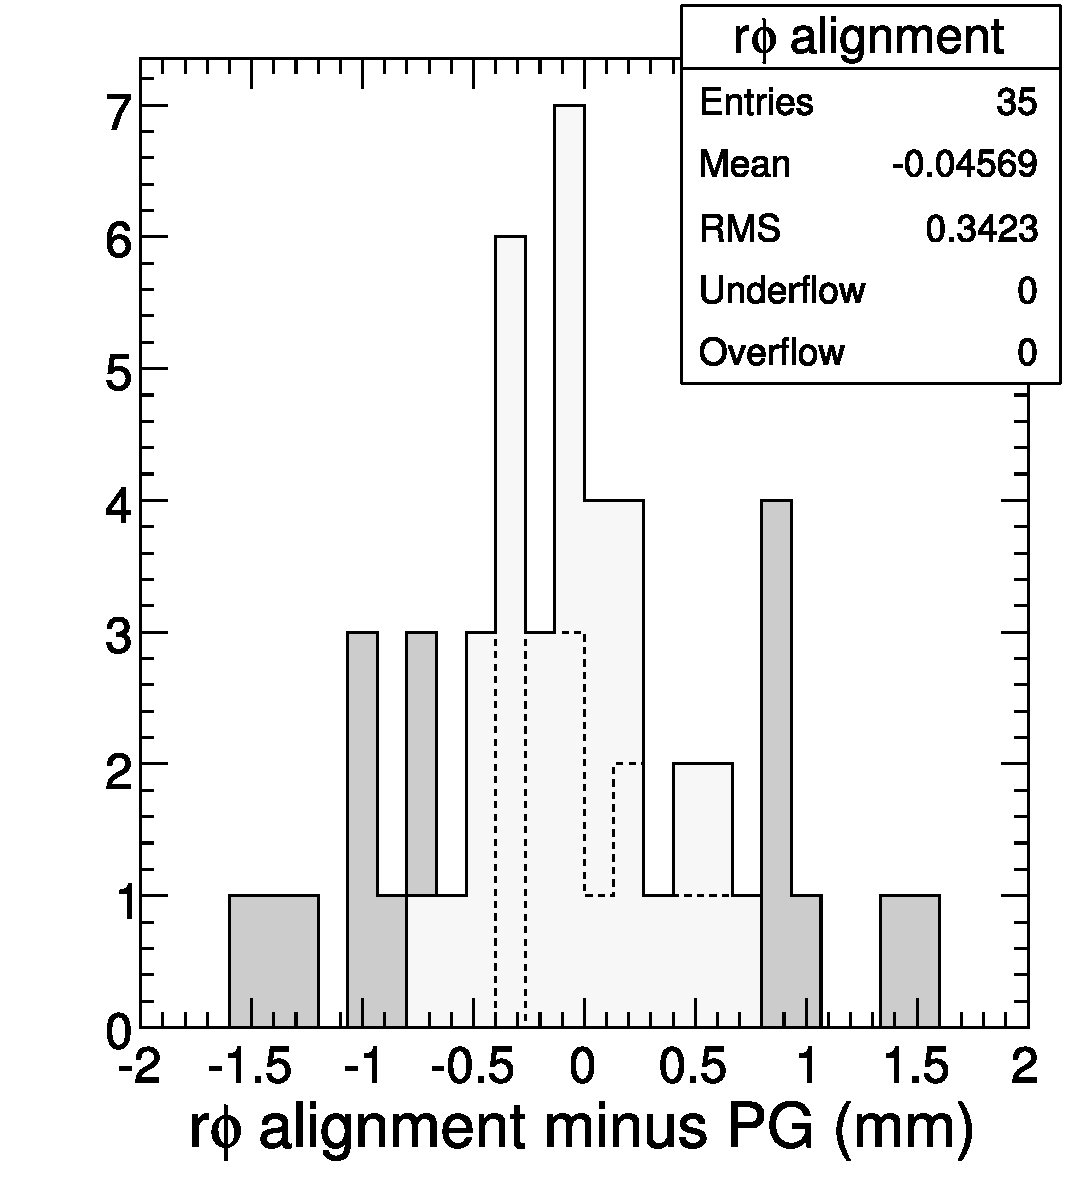
\includegraphics[width=0.35\linewidth]{plots/csc_overlaps_alignment/delta_translations_goodcolors.pdf} 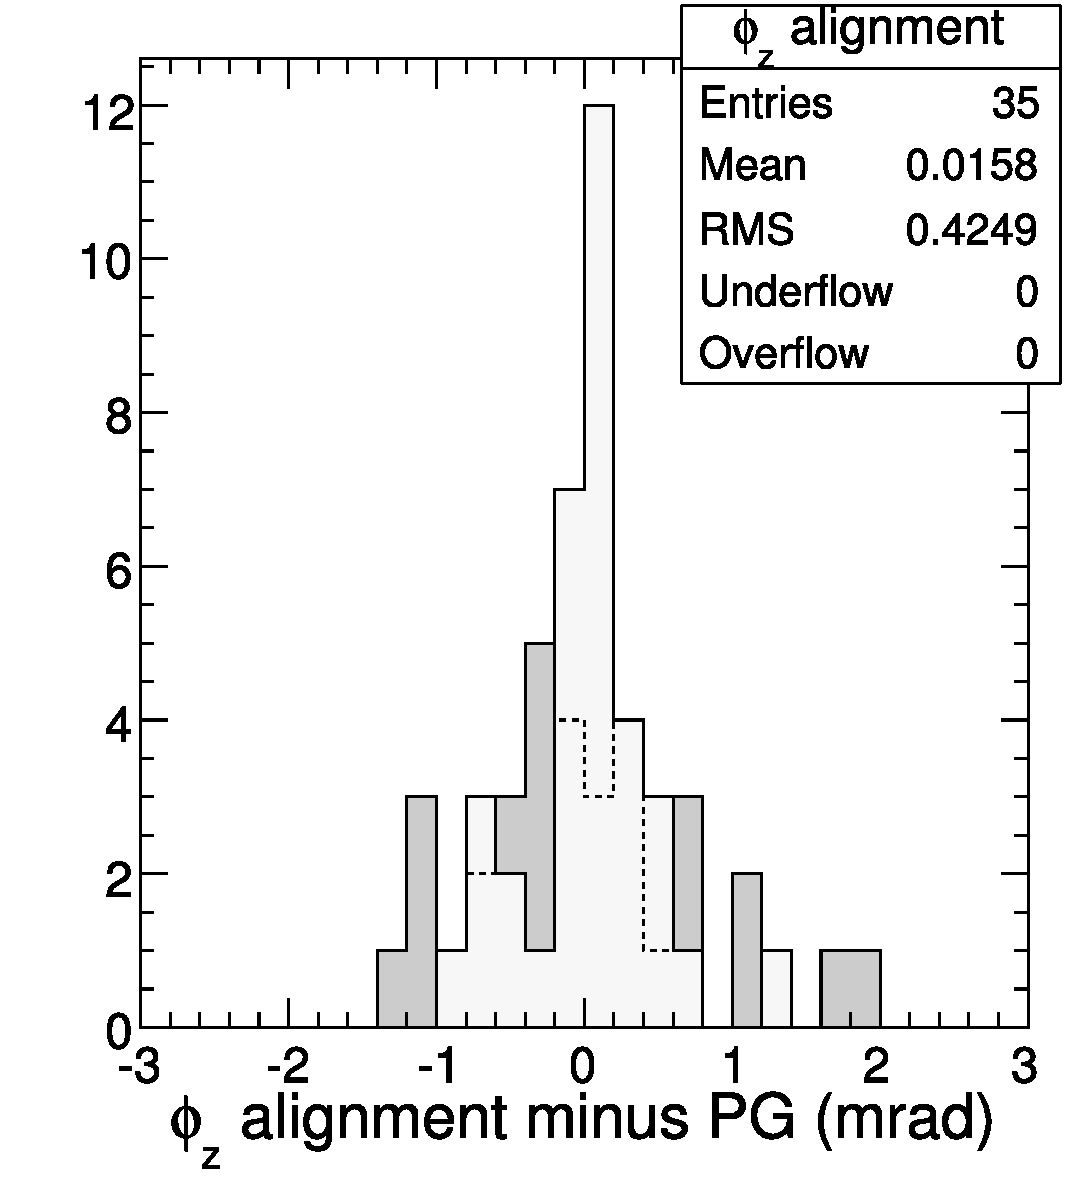
\includegraphics[width=0.35\linewidth]{plots/csc_overlaps_alignment/delta_rotations_goodcolors.pdf}
\end{center}
\caption{Chamber-by-chamber verification of the beam-halo alignment with photogrammetry.  The dark histogram is before alignment; the light histogram and statistics box are after alignment. \label{fig:overlaps_data2}}
\end{figure}

%% \begin{figure}
%% \begin{center}
%% 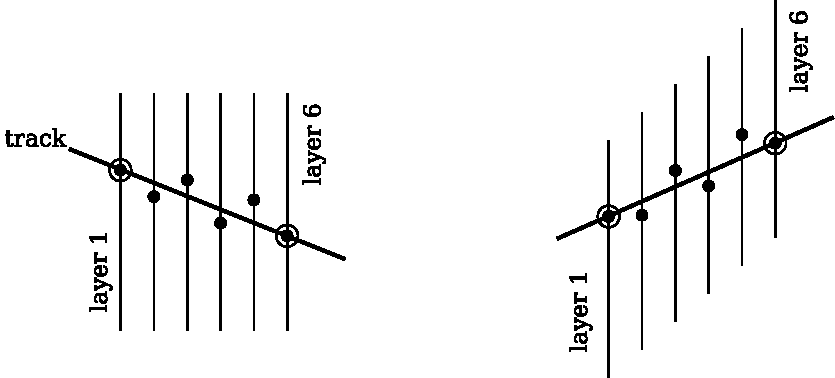
\includegraphics[width=0.75\linewidth]{plots/csc_overlaps_alignment/layer_alignment_skew.pdf}
%% \end{center}
%% \caption{Even when a track is constrained to two only layers, the positions of the other layers can only be determined up to a collective offset and a collective skew.  The two situations depicted here are indistinguishable. \label{fig:layer_alignment_skew}}
%% \end{figure}

%% \begin{figure}
%% \begin{center}
%% 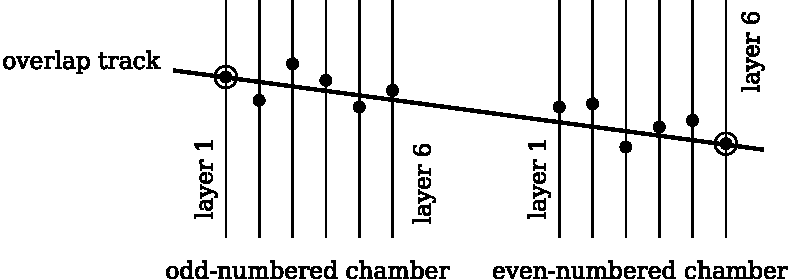
\includegraphics[width=0.75\linewidth]{plots/csc_overlaps_alignment/layer_alignment_noskew.pdf}
%% \end{center}
%% \caption{Method for aligning layers within chambers: constrain a linear track to the first and last layers in a two-chamber overlap, then align the remaining layers to that track. \label{fig:layer_alignment_noskew}}
%% \end{figure}

%% \begin{figure}
%% \begin{center}
%% 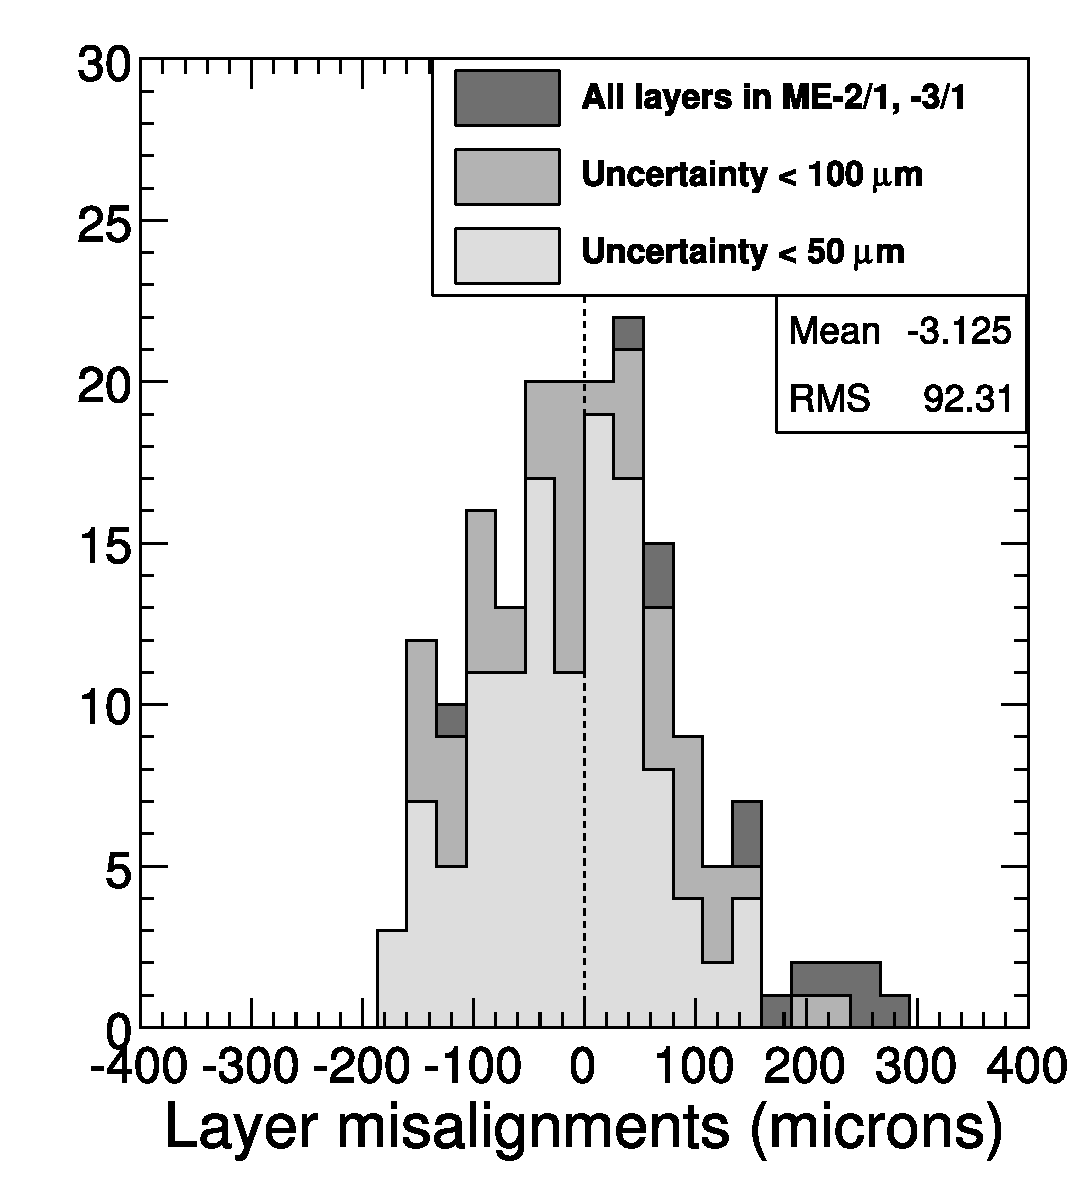
\includegraphics[width=0.5\linewidth]{plots/csc_overlaps_alignment/layer_hist.pdf}
%% \end{center}
%% \caption{Layer alignment results in ME$-$2/1 and $-$3/1, excluding layers fixed by definition. \label{fig:layer_hist}}
%% \end{figure}
